\documentclass[tikz]{standalone}
% \usetikzlibrary{arrows}
% \usetikzlibrary{calc}

\usepackage{newtxtext,newtxmath}

%!TEX root = main.tex

% mytikzset
\usepackage{tikz}
\usetikzlibrary{positioning,arrows,shapes,patterns}
\usetikzlibrary{decorations.pathmorphing}
\usetikzlibrary{decorations.markings}
\usetikzlibrary{decorations.pathreplacing}
\usetikzlibrary{calc}
\usetikzlibrary{patterns}
\usetikzlibrary{decorations.markings}
\usetikzlibrary{petri}

\tikzset{
  vector/.style={thick,double,draw=black, postaction={decorate},
    decoration={markings,mark=at position .6 with {\arrow[black,scale=0.4]{triangle 45}}}},
  axial/.style={thick,double,densely dashed,draw=black, postaction={decorate},
    decoration={markings,mark=at position .6 with {\arrow[black,scale=0.4]{triangle 45}}}},
  gluon/.style={decorate, draw=black,
    decoration={coil,aspect=0.3,segment length=5pt,amplitude=3pt}},
  pseudo/.style={thick, dashed, draw=black, postaction={decorate},
    decoration={markings,mark=at position .6 with {\arrow[red,scale=0.5]{triangle 45}}}},
  scalar/.style={thick,draw=black, postaction={decorate},
    decoration={markings,mark=at position .6 with {\arrow[black,scale=0.5]{triangle 45}}}},
  cut/.style={draw=black, decorate, decoration={snake, segment length=1mm, amplitude=0.2mm}}
}

\definecolor{myGreen}{RGB}{0,127,0}

\begin{document}
\nopagecolor
  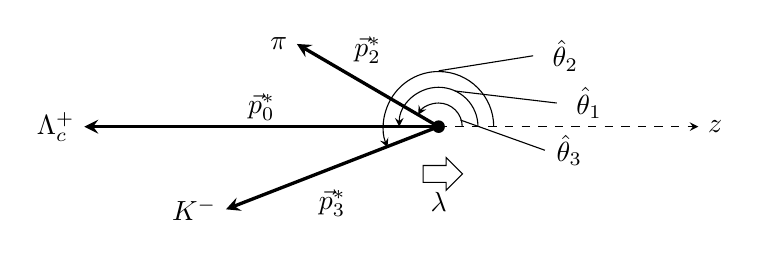
\begin{tikzpicture}[x=15mm,y=15mm]

    \coordinate[label=left:{$\Lambda_c^+$}] (Ls) at (-3,0);
    \coordinate[label=left:{$\pi$}] (Pi) at (-1.2,0.7);

    \coordinate[label=right:{$z$}] (z) at (2.2,0);
    \coordinate[label=left:{$K^-$}] (K) at (-1.8,-0.7);
    % \path let \p1=(Ls) in coordinate[label=right:{$z$}] (z) at (-\x1,-\y1);
    % \path let \p2=(Pi) in coordinate[label=left:{$K$}] (K) at ((\x2,-\y2)+(1.1,0));

    \draw[arrows={-stealth}, thin, dashed]  (0,0) -- node[] {} (z);
    \draw[arrows={-stealth}, very thick] (0,0) -- node[label={above,yshift=-2mm}:{$\vec p_0^*$}] {} (Ls);
    \draw[arrows={-stealth}, very thick] (0,0) -- node[label=above:{$\vec p_2^*$}] {} (Pi);
    \draw[arrows={-stealth}, very thick] (0,0) -- node[label=below:{$\vec p_3^*$}] {} (K);

%    \def\c0x{-1.2};
%    \def\c0y{0.6};
    % \draw[<->]  (-1.1,0.4) node[above] {\scriptsize$z$} -- ++(-0.4,0) node[] (C) {} --  +(0,0.4) node[right] {\scriptsize$x$};
    % \draw[fill=white] (C) circle (1.5pt) node[left] {\scriptsize$y$};
    % \draw[fill] (C) circle (.4pt);

    \draw[thin,arrows={-stealth}] (3mm,0mm) arc (0:150:3mm) node at (40:2mm) (A) {};
    \draw[thin,arrows={-stealth}] (5mm,0mm) arc (0:180:5mm) node at (80:4.75mm) (B) {};
    \draw[thin,arrows={-stealth}] (7mm,0mm) arc (0:202:7mm) node at (100:7mm) (C) {};

    \draw[] (B) -- (1.0, 0.2) node[label=right:{$\hat\theta_1$}] {};
    \draw[] (A) -- (0.9,-0.2) node[label={right,xshift=-1mm}:{$\hat\theta_3$}] {};
    \draw[] (C) -- (0.8, 0.6) node[label={right}:{$\hat\theta_2$}] {};

    \node at (0,-0.4) [draw=black, single arrow, minimum height=5mm,  inner sep=1mm, single arrow head  extend=1mm, label=below:{$\lambda$}] {};

    \fill[black] (0,0) circle (0.8mm);

  \end{tikzpicture}
\end{document}
